\problemname{Bonsai}

De fleste, der dyrker bonsai, siger at de gør det, fordi det er »vanskeligt« eller »harmonisk«.
Det er nu ikke derfor, Torstina gør det.
Hun vil bare score kassen på at sælge træerne, så hun får råd til at købe en masse jamaicaæbler.
Hun har lige sat en ny knold i jorden, mens hun drømmer om næste jamaicaæble.
Hvor mange år skal hun mon vente, til hun har fremavlet det bonsaitræ, hendes kunde ønsker sig?

Bonsaitræer består af $2\leq N \leq 10^5$ knolde og $N-1$ grene.
Knuderne er nummereret fra $0$ til $N-1$. 
Alle bonsaitræer begynder med en lille knold, som man sætter ned i jorden.
Hvert år vokser der en ny gren ud fra hver knold, og i grenens ende dannes en ny knold.
Man kan klippe grene af træet når som helst. 
Torstina minder dig om, at det ikke spiller nogen rolle, hvor i træet roden sidder.

Givet kundens beskrivelse af et træ, hvor mange år skal Torstina vente, inden hun har fremavlet sådan et træ?

\section*{Indlæsning}

Første linje indeholder et heltal $2\leq N\leq 10^5$, antallet af knolde i kundens ønskede bonsaitræ.
De næste $N$ linjer beskriver bonsaitræet på følgende måde:
På linje $i$ står først et heltal $0 < m_i < N$, antallet af grene udgående fra den $i$te knold. 
Derefter følger $m_i$ heltal, som angiver de knolde, der sidder sammen med den $i$te knold.

\section*{Udskrift}
Et heltal $A$: antallet af år det tager Torstina at fremavle det bonsaitræ, som kunden beskriver.

\section*{Pointsætning}

Din løsning bliver testet på en række testfaldsgrupper.
For at få point for en gruppe, skal du klare alle test i gruppen. 

\noindent
\begin{tabular}{| l | l | l |}
\hline
Gruppe & Pointværdi & Begrænsninger \\ \hline
1      &  9         & $m_i\leq 2$, det er bedst at lade træet gro fra knude~0.\\ \hline
2      & 11         & $m_i \leq 3$, det er bedst at lade træet gro fra knude~0. \\ \hline
3      & 18         & $A \leq 15$, det er bedst at lade træet gro fra knude~0. \\ \hline
4      & 22         & Det er bedst at lade træet gro fra knude~0. \\ \hline
5      & 12         & $N \leq 250$. \\ \hline
6      & 28         & Ingen yderligere begrænsninger. \\ \hline
\end{tabular}

\section*{Forklaring af eksempel 1}
Torstina kan fremavle træet på to år ved at lade det vokse som i nedenstående figur.

\begin{figure}[h]
	\centering
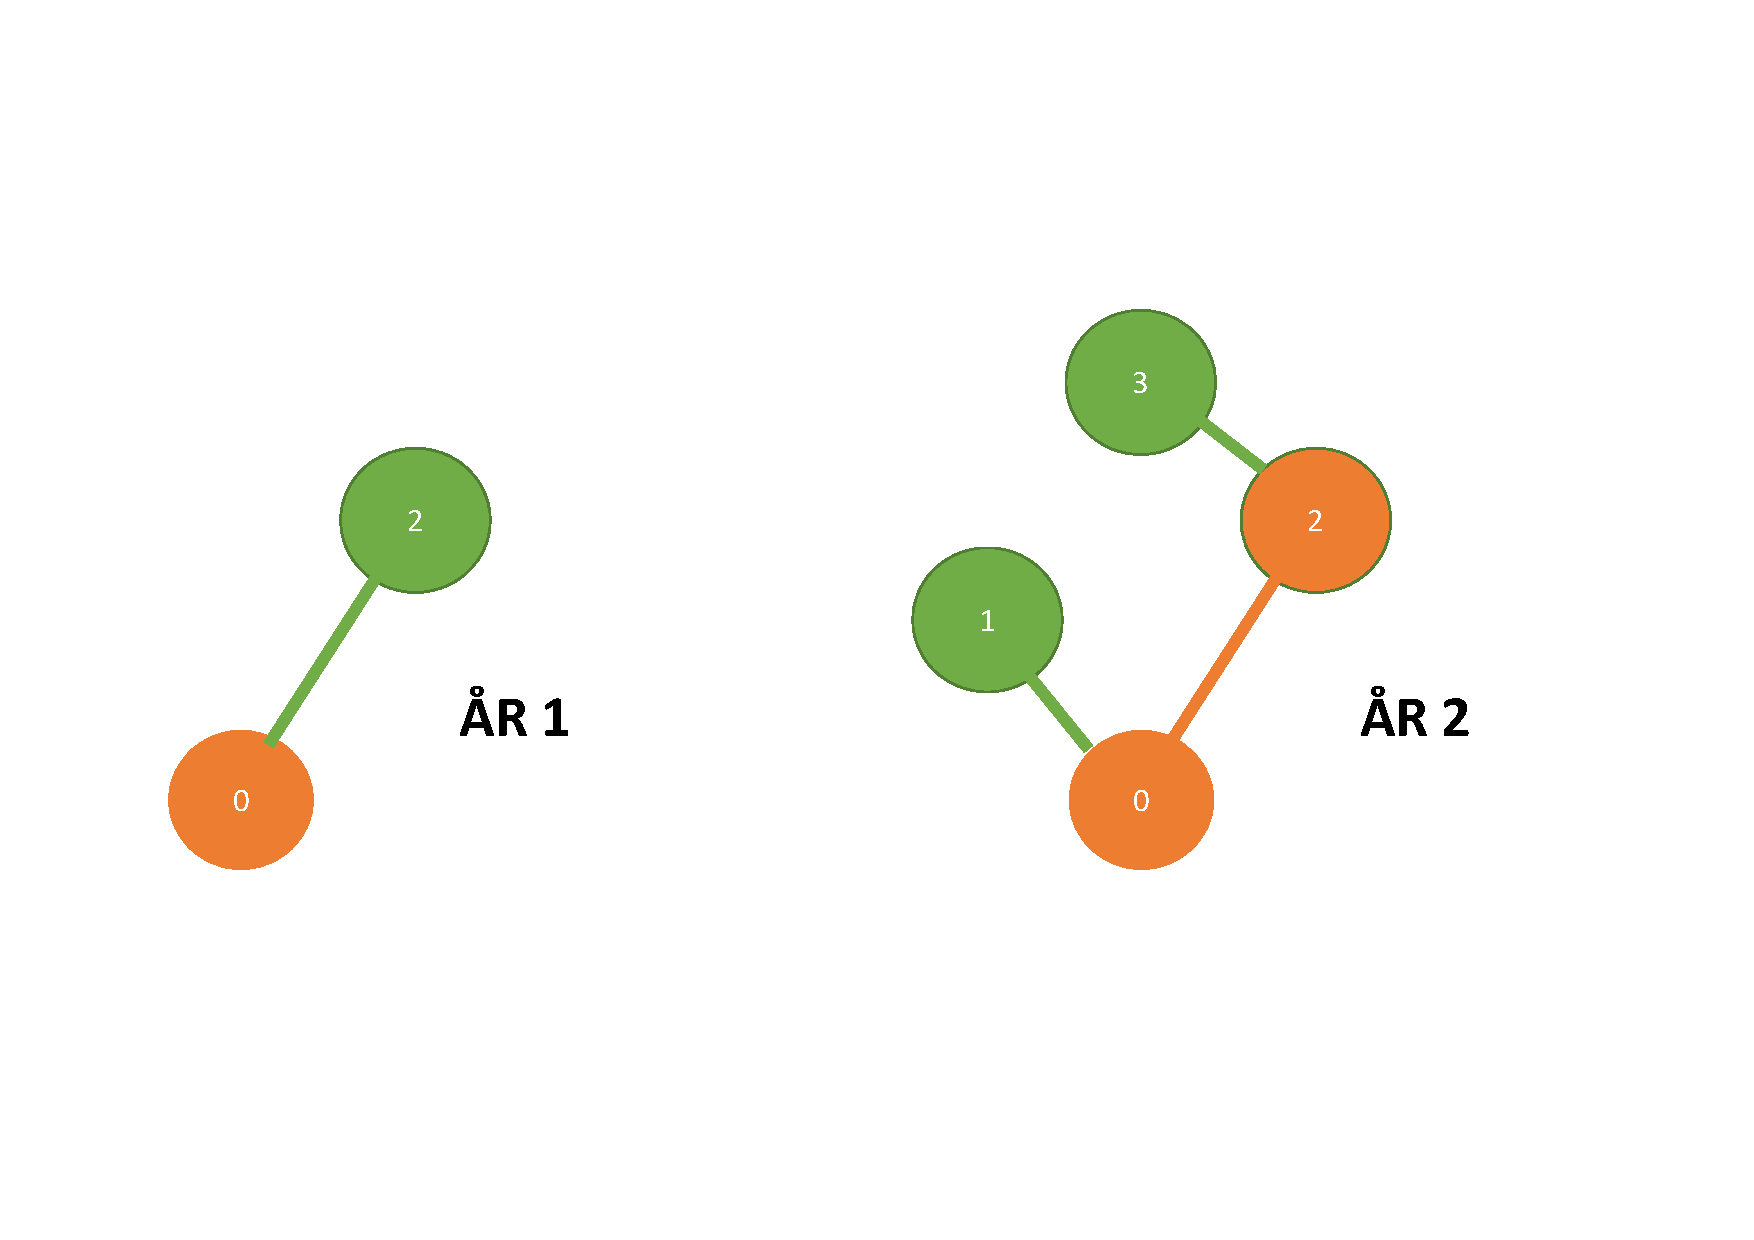
\includegraphics[width=0.5\textwidth]{Bonsai_tree}
\caption{En af de to måder man kan fremavle bonsaitræet i eksempel  1 på to år.}
\end{figure}
